% !TEX root = 0_main.tex
\chapter{Introduction}
%what are SFE and GC
\acrfull{sfe} allows two or more mutually suspicious parties to evaluate an arbitrary function on their private data.
The parties learn the output of the function without revealing any information about their private data.
An important special case of \acrshort{sfe} is its two-party version.
Formally in two-party \acrshort{sfe}, \textit{Alice} and \textit{Bob} wish to find the output of $f(a, b)$ where $a$ is Alice's private input, $b$ is Bob's, and $f(\cdot,\cdot)$ is an arbitrary function.
By far the most promising and efficient solution for two-party \acrshort{sfe} is \acrfull{gc} protocol proposed by Andrew C. Yao \cite{yao1986generate}.
In Yao's \acrshort{gc} protocol, the function $f(\cdot,\cdot)$ is represented as a Boolean circuit consisting of binary gates (e.g., AND, OR, XOR, etc.).
In this protocol, Alice encrypts (garbles) the Boolean circuit, sends it to Bob, and then Bob decrypts (evaluates) the circuit to learn the output.
The intermediate values along with the inputs are encrypted such that the parties' inputs remain private.
Secure evaluating of a Boolean circuit can also be generalized to multi-party \acrshort{sfe} \cite{goldreich1987play, ben2008fairplaymp}.

%What has been done?
A host of privacy preserving and security critical applications can directly benefit from a practical and efficient realization of \acrshort{sfe}, including but not limited to: biometrics matching, face recognition, image/data classification, electronic auctions and voting, remote diagnosis, secure search, and stable matching \cite{riazi2017toward, zhang2016robust, bringer2013privacy, evans2011efficient, barni2009secure, naor1999privacy, brickell2007privacy, jha2008towards}.

\section{Challenges}
While the \acrshort{gc} protocol was considered to be prohibitively expensive and practically infeasible a decade ago, today we are witnessing a surge of theoretical, algorithmic, and tool developments that have significantly improved the efficiency and practicality of this protocol, see \cite{malkhi2004fairplay, kolesnikov2008improved, pinkas2009secure, huang2011faster, bellare2013efficient, zahur2015two, zahur2015obliv, liu2015oblivm}.
However, three main challenges have yet to be addressed for a wide adoption of the \acrshort{gc} protocol: efficiency, scalability, and ease-of-use.

\subsection{Efficiency}
Although the \acrshort{gc} protocol has a constant round complexity which makes it superior to other \acrshort{sfe} solutions, \acrshort{gc} is still considered communication-intensive (i.e., a large quantity of data has to be transfered between parties).
It has been shown that the cost of communication is \acrshort{gc}'s performance bottleneck \cite{}.
In \acrshort{gc}, the communication is mainly originated from transferring encrypted (garbled) gates of the Boolean circuit from Alice to Bob.
To improve the efficiency of a function's secure computation, the communication has to be decreased.
This can be achieved through reducing either the communication cost of a gate, or total number of gates in the function's Boolean circuit.

The research on the efficiency of the \acrshort{gc} protocol can be roughly classified into two categories:
(i) Optimizations of cryptographic constructs and protocols such as \cite{kolesnikov2008improved,pinkas2009secure,bellare2012foundations,bellare2013efficient,kolesnikov2014flexor,zahur2015two}, out of which, the two most prominent are: Free-XOR \cite{kolesnikov2008improved} and Half Gate \cite{zahur2015two}.
Free-XOR shows that XOR gates in the circuit do not need to be communicated.
Half Gate reduces the communication cost of non-XOR (non-free) gates and provides the minimum cost that can be achieved using symmetric encryption.
(ii) Engineering techniques including but not limited to \cite{henecka2010tasty,huang2011faster,henecka2013faster,kreuter2013pcf,franz2014cbmc,mood2016frigate}.
The main objective of such work was, given a function, generating a Boolean circuit with minimum number of gates which translates directly into minimum communication for secure evaluation of that function.
They either employ library-based \cite{huang2011faster,malka2011vmcrypt,henecka2013faster} or compiler-based approaches \cite{malkhi2004fairplay,kreuter2012billion,kreuter2013pcf,franz2014cbmc}.

library-based approach is based on building a custom library for a general purpose programming language such as Java along with functions for emitting the circuit, e.g., \cite{huang2011faster,malka2011vmcrypt,henecka2013faster}.
For better usability, these libraries typically include frequently used modules such as adders and multipliers.
However, library-based approaches require do not perform global circuit optimization.

The second approach is compiler-based in which a new compiler is developed for a higher-level language that translates the instructions into the Boolean logic, e.g., \cite{malkhi2004fairplay,kreuter2012billion,kreuter2013pcf,franz2014cbmc}.
As we elaborate in the evaluation (see \chap{chap:eval}), the existing approaches do not generate the smallest possible circuit for a given function.

\subsection{Scalability}
Both library-based and compiler-based approaches suffer from complicated memory-management when the number of gates is large, thereby affecting their performance and scalability \cite{henecka2013faster, kreuter2013pcf}.
A number of compiler- and library-based frameworks have been recently proposed to address the scalability problem of previous methods by generating and secure evaluation of large circuits such as \cite{malka2011vmcrypt, mood2012memory, kreuter2012billion, kreuter2013pcf}.
However, they do not provide a generic solution that addresses both efficiency and scalability at once.

\subsection{Ease-of-use}
As mentioned earlier, GC requires the function to be represented as a Boolean circuit.
Usually, user finds it cumbersome to create a fairly simple function by connecting Boolean gates.
Library-based frameworks provide more high-level modules but user need to through knowledge about the circuit and has to manually connects different modules to create a circuit.
To simplify developing application for sfe, a number of GC framework provides user with a high-level domain-specific language to develop the function \cite{mood2012memory,kreuter2012billion,kreuter2013pcf,liu2015oblivm}.
In these high-level compiler-based framework, user's high-level code is compiled using a custom compilers in to Boolean circuits.
A major disadvantage of these method is that user has to program in a new domain-specific language.
Recently, a few gc frameworks support standard high-level language like C as well \cite{holzer2012secure, franz2014cbmc, zahur2015obliv, mood2016frigate} but the generated circuits include more gates to compared to other methods.

\section{Our Approach}
Our approach has three main pillars to address the major challenges of wide adoption of gc: gc synthesis and sequential gc and garbled processor.

\subsection{GC Synthesis}
Our gc synthesis solution simply views the circuit generation for \acrshort{gc} as an atypical logic synthesis task that, if properly defined, can still be addressed by conventional hardware synthesis tools.
By posing the circuit generation for Yao's protocol as a hardware synthesis problem, we naturally benefits from the elegant algorithms and powerful techniques already incorporated in existing logic synthesis solutions, see, \cite{sentovich1992sis,micheli1994synthesis,devadas1994logic,brayton1987mis}.
This view provides a radically different perspective on this important problem in contrast to the earlier work in this area that attempted to generate circuits by building new libraries for general purpose languages such as Java \cite{huang2011faster,malka2011vmcrypt}, custom compilers such as \cite{kreuter2013pcf,franz2014cbmc}, or introduction of new programming languages such as \cite{malkhi2004fairplay,rastogi2014wysteria}.

We introduce new techniques for minimizing the number of non-XOR gates which directly results in reduced computation and communication required for the \acrshort{gc} protocol.
We do so by integrating the cost function in the new custom libraries that we design and use within our logic synthesis flow.
This way, we are able to gain up to $80\%$ improvement in the number of non-XOR gates for benchmark circuits compared to \gls{pcf} \cite{kreuter2013pcf}.
Our methodology is automated, i.e., the savings can be achieved for many functions synthesized by our method, regardless of their sophistication.

Our GC Synthesis method can be extended to other circuit-based protocol with small changes.
Demmler et al, showed how our synthesis method can be adopt and applied for GMW where the cost depends on both depth and size of the circuit~\cite{demmler2015automated}.
In this thesis, we focus on only the solutions for the \acrshort{gc} protocol, as I believe it is the most promising generic solution for two-party SFE.

\subsection{Sequential GC}
To address the scalability we introduce sequential gc which differentiates our methodology from the previous work.
Sequential gc allows expressing the function in a very compact format, namely as a sequential logic.
The earlier work in this area mainly described functions in a combinational format, where the value of the output is determined entirely by the circuit inputs.
This input/output relationship can be expressed by a (combinational) Boolean function and a directed acyclic graph (DAG) of binary gates.
The sequential circuit description, on the other hand, allows having feedback from the output to the input by adding the notion of a state (memory).
At each \emph{sequential cycle}, the output of the circuit is determined by the current state of the system and the input.
For each particular sequential cycle, the relationship between the output and the inputs for the given states can be determined as a Boolean combinational logic.

The only previous work we are aware of which implicitly hinted at the possibility of having a more compact representation is \gls{pcf} \cite{kreuter2013pcf}.
It does so by embracing loops and unrolling them only at runtime.
A sequential circuit, however, goes far beyond the loop embracing performed at the software level.
Not only does our approach embrace the high-level loops, it also enables the user to further compact the functions by folding the implementation up to its basic elements.
For example, using our method, user can compress the 1024-bit addition function into only a 1-bit adder.

An important advantage of our sequential representation is providing a new degree of freedom to the user to fold the functions to simpler computing elements; i.e., the user has the freedom to choose the number of sequential cycles needed for evaluation of the function--the size of the combinational logic path between the states/inputs and the outputs.
The number of gates in the sequential circuit can be managed by varying the number of cycles.
The memory footprint of the \acrshort{gc} operation is directly related to the number of gates in the sequential circuit; at any moment during garbling, only the information corresponding to the current cycle needs to be stored.
Compact sequential circuits yield a small enough memory footprint that can fit mostly on a typical processor cache.
This helps us to avoid costly cache misses while accessing the wire labels during the \acrshort{gc} protocol.
Indeed, \gls{tinygarble} can enable practicable embedded implementations with a small memory footprint.

\subsection{Garbled Processor}
\subsection{Garbled Processor for PF-SFE}
The sequential representation enables, for the first time, implementation of a universal processor for private function evaluation where the function is known only to one party.
We reduce \acrfull{pf-sfe} to general \acrshort{sfe} by secure evaluation of a general-purpose processor like \gls{mips}.
\acrshort{pf-sfe} is useful for scenarios where the function is proprietary or classified, e.g., credit checking or private database queries.
The \textit{garbled processor} accepts binary code of the private function as input.
The private function can be written in a high-level language and compiled using standard compiler into the binary code.
Since a processor is inherently a sequential circuit, it was infeasible to be realized with conventional \acrshort{gc} frameworks.

\subsection{Garbled Processor for SFE}
We noticed that the garbled processor beside solving pf-sfe may also make developing sfe applications easier and more accessible to non-expert users.
Secure evaluation of standard processor like mips allows users to develop program in high-level language and compile it into binary code using standard compiler (GNU gcc).

Secure evaluation of a processor always hides the input function.
This phenomena results in a tremendous cost compared with secure evaluation of the Boolean circuit representing the same function under sfe assumption.
Thus, using garbled processor incurs an unnecessary overhead for numerous applications in which a private function is not required.
We propose two solutions for garbled processor for sfe: an extension of garbled mips for \acrshort{sfe} and ARM2GC framework which is based on ARM processor.

\subsubsection{MIPS for SFE}
We extend garbled mips to provide a generalized support for \acrshort{sfe} of varying flavors of privacy, beyond \acrshort{pf-sfe}, to allow for more relaxed privacy demands and hence an improved performance.
More explicitly, the parties can evaluate a private, semi-private or public function by revealing none, partial or all information about the function respectively while still benefiting from the simplicity of programming a processor.
We provide a coarse-grain optimization in which both parties decide first which subset of mips ISA they are willing to use which determines the level of privacy ensured.
The function is compiled from a high-level language, e.g., C/C++ into assembly code of the agreed upon ISA. Next, the garbled processor is securely evaluated given users' garbled input and the compiled function instructions (also garbled) to compute the output.

\subsubsection{ARM2GC}
We also introduce a methodology to perform fine-grain (gate-level) optimization on garbled processor such that only the gates associated to the private inputs incur garbling cost.
Our key observation is that the gates whose outputs are independent of the private data (and thus known to both parties) can either be computed without communication and encryption or simply skipped.
This observation gives birth to the novel \gls{skipgate} algorithm.
The algorithm wraps around the \acrshort{gc} protocol to compute the gate outputs that can be computed without communication and to mark the redundant gates for skipping\footnote{\gls{skipgate} avoids garbling redundant gates and is orthogonal to cryptographic methods such as Free XOR~\cite{kolesnikov2008improved} and Half Gate~\cite{zahur2015two} that reduce the garbling cost of a gate.}.

\gls{skipgate} is mostly effective for reducing the garbling cost of sequential circuits containing known control paths.
An example of such a circuit is the garbled processor where the control path depends on the binary code of the function that is known to both parties.
By utilizing this property, we develop a high-level \acrshort{gc} framework called \gls{arm2gc} built upon the \gls{arm} instruction set and the \gls{skipgate} algorithm.
Users can develop the secure function in high-level languages, e.g., C/C++ and compile it using standard \gls{arm} cross-compilers.
In contrast to the earlier custom high-level compilers which called for new ad-hoc verification techniques~\cite{rastogi2014wysteria,demmler2015aby,liu2015oblivm,mood2016frigate}, \gls{arm2gc} inherits the \gls{arm}'s available fully verified compilers.
Thanks to \gls{skipgate}, \gls{arm2gc} incurs a garbling cost comparable to the \acrshort{hdl} synthesis approach of \gls{tinygarble} while allowing users to develop \acrshort{sfe} applications in a high-level language.

Our work leverages \gls{arm} as the general purpose processor because of \gls{arm}'s pervasiveness and, most importantly, conditional execution.
The latter simplifies the framework by reducing conditional branches and making the program flow predictable for both parties to take the full advantage of the \gls{skipgate} algorithm.
We modify the standard \gls{arm} architecture (without affecting the instruction set) such that \gls{skipgate} is more effective on the circuit.

\section{Contributions}
In brief, the main contributions of this thesis are as follows:
\begin{itemize}
  \item
  We address the efficiency challenge of the gc protocol by introducing TinyGarble GC synthesis by adapting the established \acrshort{hdl} synthesis techniques to compile and optimize a function into a netlist of gates for use in secure computation protocols.
  \item
  We address the scalability challenge of the gc protocol by introducing TinyGarble Sequential GC that allows us to achieve an unprecedented compactness in function representation and memory footprint at the same time using the same GC synthesis method.

  \item
  We implement the first scalable emulation of a universal processor for private function evaluation where the number of instruction invocations is not limited by the memory required for garbling.
  This design is uniquely enabled by the \gls{tinygarble} sequential GC.
  Our design is a secure general purpose processor based on the \gls{mips}~I instruction set that receives as inputs the private function from one party and the data from the other.

  \item
  We propose the solution for 2-party \acrshort{gc}-based secure sequential function computation with different \acrshort{sfe} flavors that allows leveraging the trade-off between privacy and performance: application-specific IS for \acrshort{sfe}, restricted IS for semi-private \acrshort{sfe}, and full IS for \acrshort{pf-sfe}.

  \item We introduce the novel \gls{skipgate} algorithm that avoids redundant garbling by utilizing the mutual knowledge between the two parties.

  \item
  We develop the \gls{arm2gc} framework based on the \gls{skipgate} algorithm and \gls{arm} processor.
  In this framework, users can efficiently develop \acrshort{sfe} applications in a high-level language like C/C++.
  It enables them to benefit from the available fully verified compilers of \gls{arm}.
  We modify the \gls{arm} architecture (without affecting the instruction set) to make it most effective for the \acrshort{gc} protocol with \gls{skipgate}.
\end{itemize}


\section{Global Flow}
\subsection{TinyGarble}
We combined our GC Synthesis and Sequential GC approach into a gc framework called \gls{tinygarble}.
\gls{tinygarble} accepts inputs in two different formats: a standard hardware description language (\acrshort{hdl}), or a higher level language as long as it is compatible with the existing high level synthesis (\acrshort{hls}) tools, e.g., the C language for  SPARK \cite{Gupta2004} and Xilinx Vivado \cite{tool:Vivado}, or Python for PandA \cite{tool:PandA}, that converts the high level language to an \acrshort{hdl}.
Beside user's manual optimization, \gls{tinygarble} performs various optimizations through standard \acrshort{hdl} synthesis tools to generate an optimized \emph{netlist}, i.e., list of gates, which is then transformed to \acrfull{sscd} format to be used with our \acrshort{gc} implementation.

The global flow of \gls{tinygarble} framework is shown in \fig{fig:tinygarbel-global-flow}.
The framework consists of two main part (i) \acrshort{gc} synthesis and (ii) \acrshort{gc} engine.
The \acrshort{gc} synthesis flow receives a function description in \acrshort{hdl} and generates a circuit description that can be efficiently evaluated by the \acrshort{gc} engine.
The \acrshort{gc} synthesis can generate combinational circuits as well as sequential ones.

The \acrshort{gc} engine allows two parties, Alice and Bob, to securely evaluate the function given the function description generated by the \acrshort{gc} synthesis flow.
The engine is an implementation of Yao's \acrshort{gc} protocol in C++ and is developed based on JustGarble \cite{bellare2013efficient}.
Our \acrshort{gc} engine supports communication which was missing in JustGarble.
It also includes implementation of Half Gate \cite{zahur2015two}, the most recent theoretical optimization on the \acrshort{gc} protocol that reduces the communication and computation cost by 33\%.
Also most importantly, our \acrshort{gc} engine supports garbling/evaluating of sequential circuits.


\begin{figure}
\centering
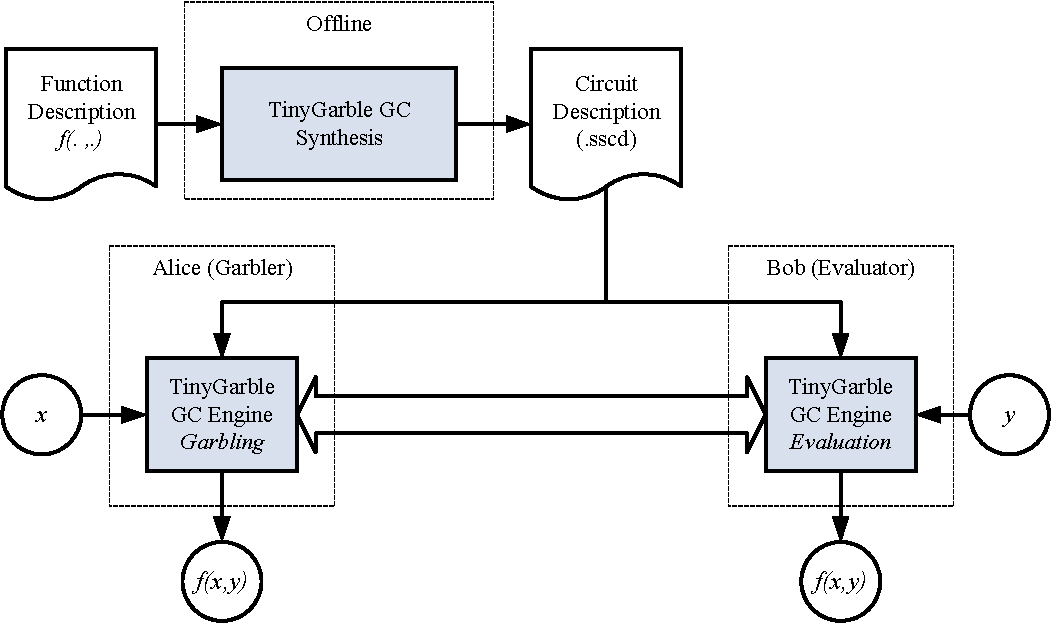
\includegraphics[width=\textwidth]{tinygarble_flow-crop.pdf}
\caption{The global flow of \gls{tinygarble} framework.
The framework consists of \acrshort{gc} synthesis flow and \acrshort{gc} engine.
The \acrshort{gc} synthesis flow generates the optimized circuit description given a function.
The \acrshort{gc} engine allows two parties (Alice and Bob) to securely compute the function according to Yao's \acrshort{gc} protocol.
}
\label{fig:tinygarbel-global-flow}
\end{figure}

\subsection{ARM2GC}
The \gls{arm2gc} framework is built upon the \gls{tinygarble} framework.
The circuit of ARM processor (notated as f()) is synthesized using the \gls{tinygarble} GC synthesis.
The function g(,) is described by user in a high-level language, e.g., C and compiled using an ARM compiler, e.g., gcc-arm to produce the binary code.
Then, the \gls{tinygarble} gc engine that supports skipgate is used to securely evaluate the ARM processor given the binary code (p), and parties inputs (a,b).
At the end both parties revives the output of $f(a,b,p) = g(a,b)$.

\begin{figure}
\centering
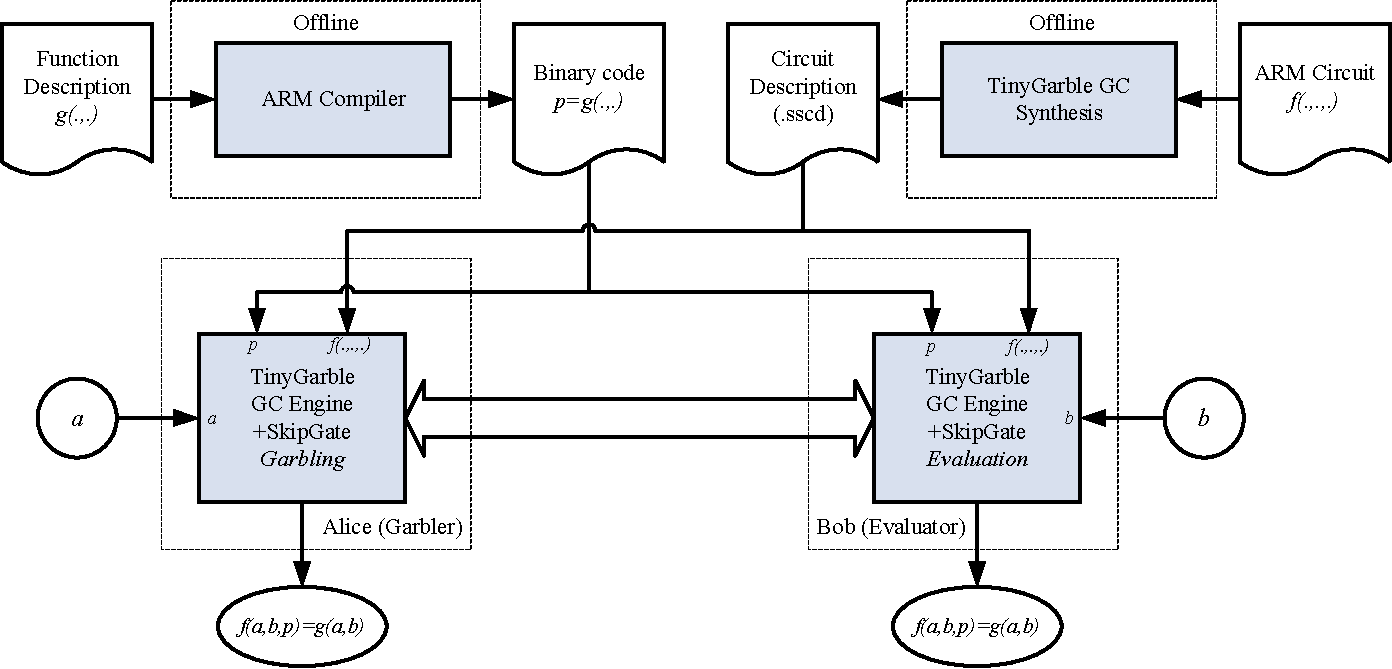
\includegraphics[width=\textwidth]{arm2gc_flow-crop.pdf}
\caption{The global flow of \gls{arm2gc} framework.
The framework consists of \acrshort{gc} synthesis flow of \gls{tinygarble} and its \acrshort{gc} engine with \gls{skipgate} algorithm.
The \acrshort{gc} synthesis flow generates the circuit description of the ARM processor $f(\cdot,\cdot,\cdot)$.
The function to be securely evaluated ($g(\cdot,\cdot)$) is compiled using an ARM cross-compiler.
The \acrshort{gc} engine allows two parties (Alice and Bob) to securely compute the ARM circuit $f(a,b,p)$ where $p$ is the binary code of $g(\cdot,\cdot)$.
At the end, they will receive the output of $f(a,b,p) = g(a,b)$
}
\label{fig:arm2gc-globalflow}
\end{figure}


\section{Organization}
The thesis is organized as follows.
We review the preliminaries and background of the sfe, gc, and Boolean circuits in \chap{chap:prelim}.
We discuss TinyGarble GC synthesis and its limitation in \chap{chap:syn}.
TinyGarble Sequential GC and its overhead is described in \chap{chap:seq}.
We introduce skipgate algorithm to remove the sequential overhead in \chap{chap:skipgate}.
Next, we present garbled processors for pf-sfe, sfe and ARM2GC framework in  \chap{chap:processor}.
Lastly, we review the related work in \chap{chap:related} and conclude the thesis in \chap{chap:conclusion}.

In \appx{chap:knn}, we implement a scalable solution for private nearest neighbor search as an application of \gls{tinygarble} sequential GC.
In \appx{chap:library}, we provide a library of \acrshort{gc} optimized circuits for complex mathematical/logical operations made by \gls{tinygarble} GC synthesis.
In \appx{chap:open-source}, we extend evaluation of \gls{tinygarble} sequential GC by comparing the result of open-source synthesis tool with commercial one.
We discuss tinygarble \acrshort{gc} engine in more details in \appx{chap:engine}.
